\documentclass[]{article}
\usepackage{amsmath,amssymb,wrapfig,lipsum,
caption,subcaption,graphicx,setspace,lmodern}
\usepackage[inner=2cm, outer=2cm]{geometry}


%-------------------------------------
%Code used to include matlab code
\usepackage{listings}
\usepackage{color}
\definecolor{betterGreen}{rgb}{0,0.5,0}
\lstset{language=Matlab, commentstyle =\color{betterGreen}, keywordstyle=\color{blue},stringstyle=\color{magenta}, showtabs=false,showspaces=false, showstringspaces=false, frame=single}
%----------------------------------

\begin{document}

\newgeometry{left=5cm,right=5cm,bottom=2cm }



\title{Interactive Visualization Software for           \linebreak Gene Network Analysis }
\author{Min Hyung (Daniel) Kang}
\date{Aug 31st, 2015}
\maketitle

\begin{center}

Advisor : Eugene Demidenko

\bigskip \bigskip \bigskip 
 \bigskip \bigskip \bigskip
 

\includegraphics[scale=0.2]{logo}
\bigskip

Department of Mathematics, Dartmouth College
 \bigskip \bigskip \bigskip 

\end{center}


\restoregeometry
\newgeometry{top=2cm,left=2cm,right=2cm,bottom=2cm}



\pagebreak

\doublespacing

\tableofcontents

\bigskip \bigskip \bigskip \bigskip

\section{Summary}

For past two months, I stayed on campus and studied application of Gene Rank, a concept introduced by Professor Eugene Demidenko of Geisel Medical School. The main goal was to develop an interactive software for studying and visualizing Gene Network. Gene rank combines \textit{a priori} knowledge of gene connectivity and microarray datasets of gene expressions, and using a recursive definition as in PageRank of Google, computes a measurement of gene's connectivity with other genes. I worked on developing a java program to visualize the connectivity and GeneRank of genes.  

\pagebreak

\section{Description}

 \textit{Microarray Enriched Gene Rank} (GR) applies the PageRank algorithm, developed by Page \textit{et al} \cite{pagerank} which ranks the webpages according to their connectivity with other pages, on gene expressions. GR combines the previously known knowledge about gene connectivity and microarray data, and is defined recursively just like the Page Rank.
 
 GR is computed using a matrix of gene expression data sets, with each row and column representing different genes and samples, respectively. As the sign of correlation does not matter, we use squared correlation coefficient, which explains how much of variations of a gene can be explained by that of the other gene. We normalize the resulting matrix so that sum of each row is 1. We compute the rank of a gene using weighted sum of squared correlations, where the rank itself is the weight (hence the recursive definition). Lastly, we add constant connectivity of 0.9 (or assumes \text{a priori} value of connectivity) to the expression. Once the equation is set up in matrices, we can obtain the values of GR by computing the maximum left eigenvector of the formulated matrix. \cite{generankdef}

The original plan before the summer term began was to look into applications of Gene Rank, such as looking at relationship of changing connectivity of TP53 and cancer development. However, near the end of spring term, Professor Demidenko suggested a topic that suited me better: visualization of the gene connectivity. As a Computer Science and Math double major, the task was much more relevant and familiar than understanding the relationship between the genes. I was to write a java program that will load dataset to create a GoogleEarth-like figure, which will display the genes, their connections and generanks. The user was to be able to navigate around and study the relationships between different genes. 

Visualization is an important aspect of data analysis. It allows us to understand the data more intuitively, so that one can comprehend the dataset better. Just as my own case, analysts of genes may not be professionals in biology or biostatistics. For such group of people, it is helpful to visualize the genes rather than read them in numerical forms. And if one is allowed an interactive visualization rather than a fixed form (such as a diagram or a table), one can focus on particular points of interest with ease. 

The problem then becomes how to visualize the earth. Constructing a sphere-like form and making camera rotate around like Google Earth is a relatively common project. Various 3-d programs these days support such transition of cameras, and moving view around a point (or sphere in our case) is one of the basic requirements of modern games. Of course, when we start taking efficiency and performance into consideration as well, the program gets a little more difficult. On that matter, Google Earth could be considered as a state of the art visualization program. It combines unimaginable amount of data and displays to the user what he/she requests to see. As one who have used the program would note, it is user friendly and so precise that concern for privacy was raised. Hence, from the beginning Google Earth was a good archetype.

However, one difference between traditional 3-d visualization problems and gene visualization is that the genes are not neatly placed on the surface of a sphere. Indeed, they have no set "location." Hence, we have to find a way to project the genes on the surface of the unit sphere without losing so much information. The problem resembles that of PCA(Principal Component Analysis) or SVM(Support Vector Machine), yet they alone are not enough to ensure sphere-shaped spread of genes. Hence, what Professor Demidenko does is use Gauss-Newton algorithm to solve non-linear least-square equations, as described in the appendix A.1.

Once we have all the points projected to the surface of the sphere, we can project them onto a 2-d plane using the methods described in appendix A.2. We have a vector that defines the angle of the viewing camera, and a plane which crosses the center of the sphere and has that vector as the normal. Using the equations used in appendix A.2, we can project the 3-d points onto this plane, which we then display on the screen. We add the earth (circle), correlation lines between the genes and Gene Rank values, which gives us a full visualization.

Once we have a fixed image, there are many attributes we can change to make it interactive. The user can click on a gene to see information about the gene as well as the genes it is connected to, a list of which can be sorted by the GeneRank, R, or the name of the genes. One can click on a correlation line between a gene that was clicked and another gene to make it permanent : that is, that correlation line is always displayed even if we click on other genes. Moving around the cursor above the correlation line will show the information regarding that line. One can double click on a spot on the earth, which will rotate to make the clicked spot as the center and zoom in a certain amount. The user can also search for a gene, and if there is a match, the image will rotate so that the gene of interest is in the center. One can also click-drag-release to rotate the earth in desired direction, and use mouse scroll to zoom in and out.   

In addition, there are filters one can apply to the display. One can choose to see the genes by setting the boundary of GeneRank, see them filtered by distance,(shows only genes with higher GR values when far away) or view all of them. One can also filter the correlation lines in a similar manner : set the boundary of R, filter by distance, or view all. User can change the values of distance, $alpha_{view},$ $beta_{view}$ and $size$ values via scrolls to change around the view. One can also click on arrow buttons to shift the view (rather than rotate) or home button to move to default view. There is also a preview panel which will display the current perspective with regards to the whole earth.

At this moment, the user has to supply 3 data files for the program : R, GR, and angle data. This can be done by running on Gene Expressions Data the R-script originally written by Professor Demidenko . Even though I could make java program to do the whole process, running r-script is much more efficient as R language and its inherent functions are optimized for statistical evaluations such as computing correlation or standard deviations. However, there is a shortcoming that one needs to have R installed in order to run this program, which partly goes against the intention of the multi-platform support of the program. There is also a way to incorporate R-code within java code, yet it also requires additional installations and complex coding that for the prototype, current implementation seems sufficient.

\section{Results}
The resulting program was written in java. It has 17 classes in total, and about 3,000 lines of code. They are structured as the following : 
\begin{figure}[h!]
	\centering
	\includegraphics[scale=0.7]{diagram}
	\caption{Structure of classes \textit{(rectangles indicate visual components, while circles indicate objects or algorithmic components)}}
\end{figure}

\singlespacing

\begin{itemize}
\item FileChooserPanel : asks the user to specify the three files to load for the program : R, GeneRank, Angle.
\item Main : Main frame that sets up all the panels.
\item LeftPanel : Left part of program which contains ScrollPanel, MovePanel, and PreviewPanel.
\item ScrollPanel : Allows user to scroll values of $distance$, $alpha_{view}$, $beta_{view}$, $size$ to change the view.
\item MovePanel : Allows user to click on arrows to move the view, or click home button to move to default view.
\item PreviewPanel : Shows the view of the user with respect to whole picture.
\item MainPanel : Main program that does all the necessary computations and displays the GeneEarth.
\item Calculator : Used by MainPanel to compute certain calculations such as projection.
\item Coordinate : Object used by program to represent a 2-d or 3-d points.
\item RightPanel : Right part of program which contains DataPanel, SearchPanel, FilterPanel and FilterRPanel.
\item DataPanel : Shows the current (clicked) gene's name and gene rank.
\item SearchPanel : Textbox where user can type in a gene's name to find the gene and see it.
\item FilterPanel : Display options to filter genes by distance, by GeneRank, or to view all.
\item FilterRPanel : Display options to filter correlation lines by their values, by distance, or to view all.
\item ListPanel : The rightmost part of the program, which shows all the genes current genes are connected to.
\item Indexer : Used by ListPanel to sort the list of genes by GeneRank or R.
\item NameIndexer : Used by ListPanel to sort the list of genes by their names.


\end{itemize}

\doublespacing
\bigskip
In terms of the actual program, the following figures 2-5 indicate the visual components of the program. There are other classes, such as Coordinate, Indexer, NameIndexer, and Calculator that do not deal with visual components and cannot be represented in the diagram. : 

\begin{figure}[h!]
	\centering
	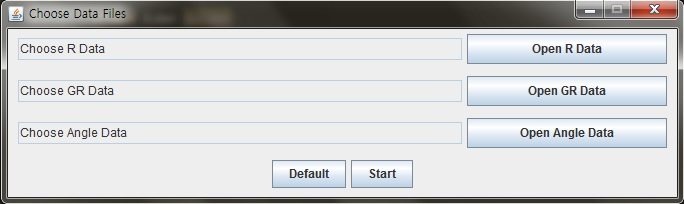
\includegraphics[scale=0.48]{FileChooser}
	\caption{FileChooserPanel}
\end{figure}

\begin{figure}[h!]
	\centering
	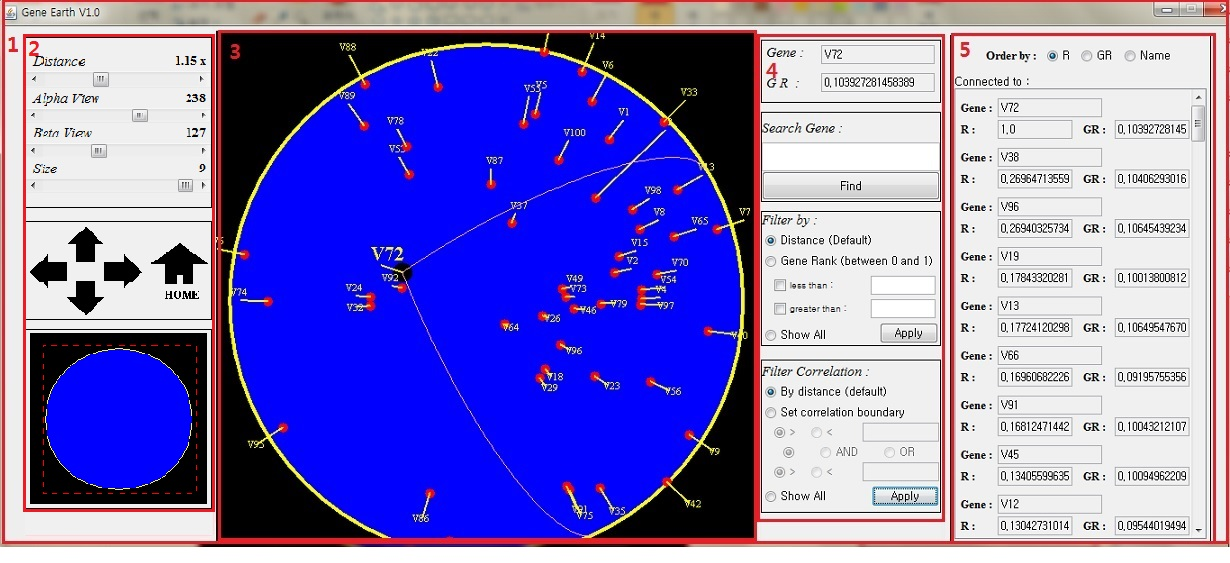
\includegraphics[scale=0.48]{ProgramPanels}
	\caption{Major classes with sample dataset of 100 genes: \textit{(1. Main 2. LeftPanel 3. MainPanel 4. RightPanel 5. ListPanel)}}
\end{figure}

\begin{figure}[h!]
	\centering
	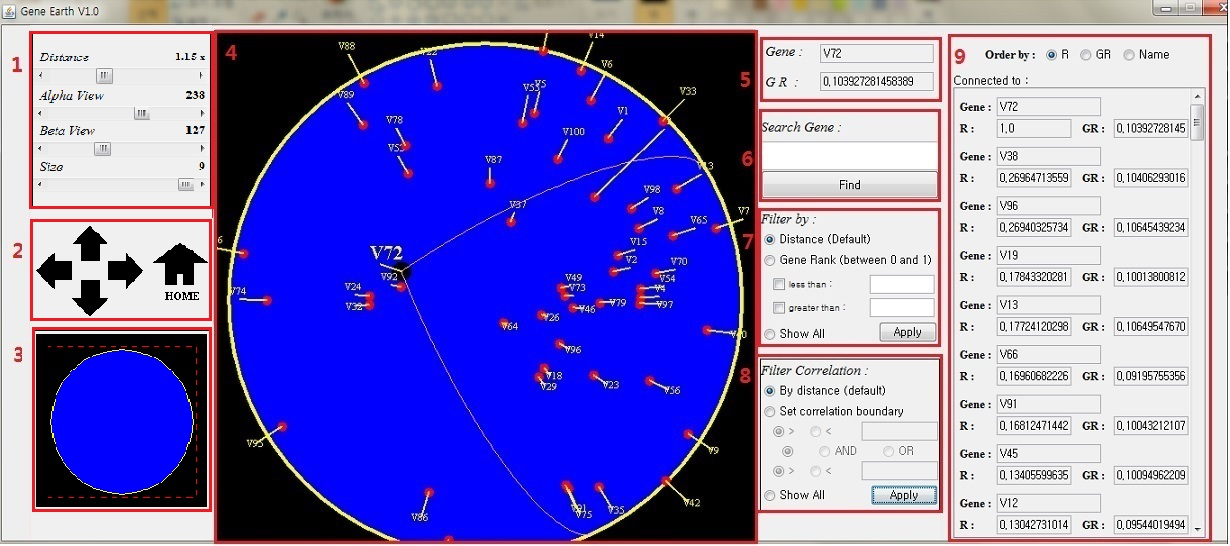
\includegraphics[scale=0.48]{ProgramPanelsDetail}
	\caption{Specific Panels with sample dataset of 100 genes: \textit{(1. FilterPanel 2. MovePanel 3. PreviewPanel 4. MainPanel 5. DataPanel 6. SearchPanel 7. FilterPanel 8. FilterRPanel 9. ListPanel)}}
\end{figure}


We can take a look at real data (a dataset with 1,500 genes) and observe the results.   Note again that the data in Figures 3-4 were sample dataset with 100 genes.

\begin{figure}[h!]
	\centering
	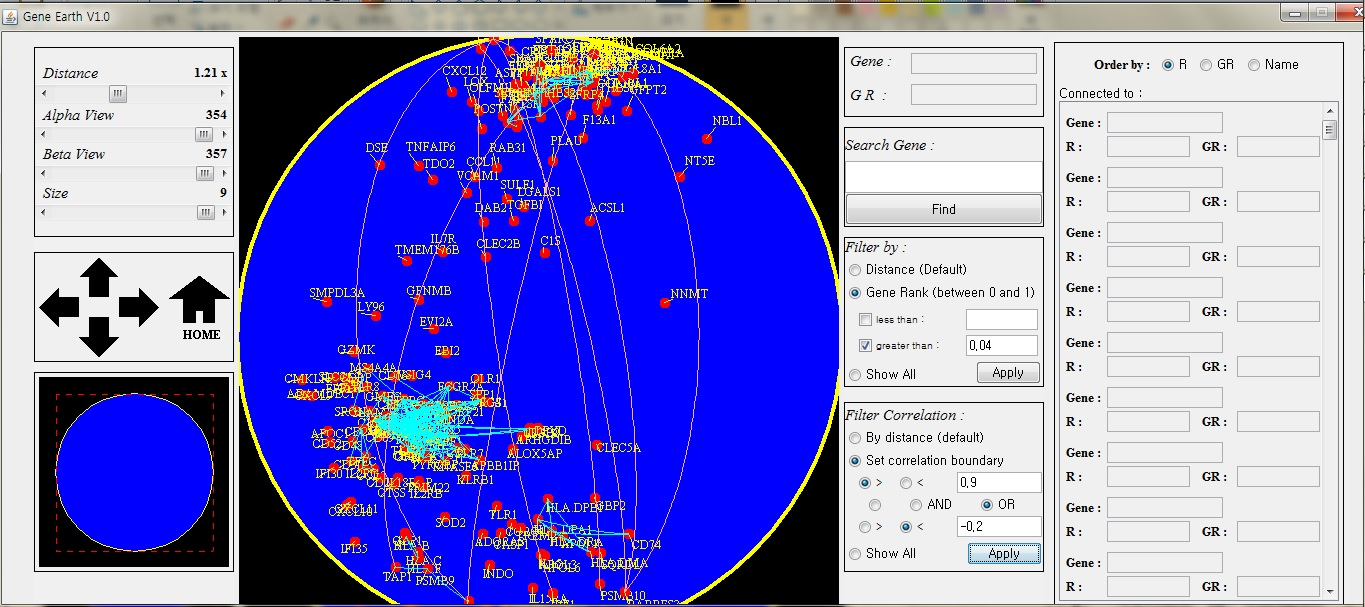
\includegraphics[scale=0.48]{RealDataExample}
	\caption{Real Data Example with 1500 genes \textit{(We can observe two major clusters of genes, one towards the top and another towards left bottom)}}
\end{figure}

\begin{figure}[h!]
	\centering
	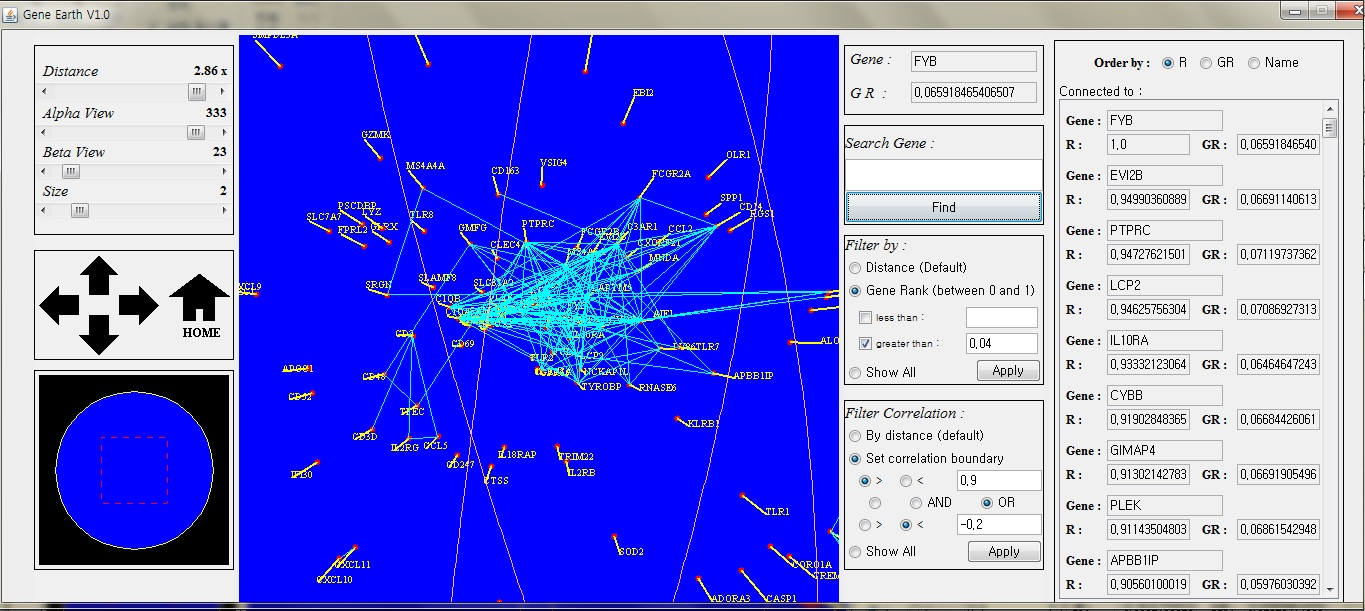
\includegraphics[scale=0.48]{RealDataExample2}
	\caption{Real Data Example with 1500 genes \textit{We zoom on the left cluster, and we see which genes are connected with high connectivity : filtered with GR \textgreater 0.04, R \textgreater 0.9 or R \textless -0.2}}
\end{figure}

The dataset that was used above was TCGA (The Cancer Genome Atlas) Gene expression data from 489 ovarian biopsies. It is a set of representative 1500 expressions chosen out of 11,864 dataset, and is the same dataset used by Professor Demidenko's paper, where he points out that classification of genes can significantly improve treatment outcomes by identifying the subtype of the cancer, and GR can be used to identify the groups.\cite{generankusage}
As portrayed in the above example, one can use this program to visually identify the connected genes and the clusters.

There are other features but they will not be covered in this summary, for I will be doing more documentation in README (as one would do for a regular program) and make a short instructional video of demo usage.

\section{Conclusion}

The program is far from being complete. There are numerous additions or renderings that could be done in terms of efficiency and precision. A few might be but not limited to: making the window resizable, rotation more precise, algorithm faster, and graphics more aesthetic. However, I believe current version to be a good prototype of an efficient platform-free program of visualization of genes. This program can help one to visually recognize the pattern or confirm the numerical association one observes from raw data. 

The research was a valuable experience in various ways. It was first independent project under guidance of professor, and I had to make design choices, find ways to implement algorithms, and even work out equations before I could program them. They were totally different from regular programming assignments in that there were no set expectations nor guidelines and no TAs to help me when I could not figure out a solution. I have regrets in terms of how I programmed some components, but I do believe it is all part of learning process. It is also noteworthy that it was my first java program in three years, meaning I had to review a lot of materials before I could sit down and start coding. I also tried to study algorithms apart from my research, and the content actually coincided a lot with the project, such as sorting and searching.

As a Computer Science and Math double major, I am considering focusing on data science. A relatively new field, data science utilizes math, statistics, and programming to gather, understand and sometimes explain the data. My research for past two months, which focused on visualization of gene connectivity, has been my first practical experience in the field. Data visualization is an important aspect, in that it involves a lot of coding as well as understanding of ways to efficiently visualize data. Dealing with big data, I had to consider memory usage as well as algorithmic efficiency, which are all important factors in the field.

Alongside research, I have also been taking data science courses from Coursera to work on my skills in R Programming. I will continue studying the field more in depth in the future. In upcoming fall, I am going on an exchange term at Aquincum Institute of Technology (AIT) in Hungary, where I will be studying computer science and entrepreneurship. I will be working as presidential scholar in winter term with professor Qiang Liu on "Machine Learning for Crowdsourcing", as well as take his course CS74 Machine Learning. As such, I have plans ahead, and I hope this research will set a good cornerstone for my future career. 

The off-term research grant I received, Kaminsky Research Fund, was used wholly for housing and meals. Along with earnings I received from TAing CS50, the grant allowed me to stay on campus and focus on research. If it had not been for the grant, I would have needed to find additional work that would fund my housing and dining, which is not trivial at all. Hence, I greatly appreciate the opportunity that was given.


\bigskip \bigskip \bigskip \bigskip

\newpage
\appendix
\singlespacing
\section*{Appendices}
\section{Visualization}
\subsection{Projection of genes to surface of  3d unit sphere}
Our goal is to project $n$ multidimensional vectors ${x_i,i=1,2,\dotsb,n}$ onto a sphere, keeping the deformation in pair-wise correlation $r_{ij}$ as small as possible. We can denote a 3-dimensional vector on the sphere as a unit vector 

\[
z_i=\left[
\begin{array}{c}
\cos \theta_i \cos \phi_i\\
\sin \theta_i \cos \phi_i\\
\sin \phi_i
\end{array}
\right]
\]
where $\theta_i$ is angle with respect to $x$ axis and $\phi_i$ is angle with respect to $z$ axis. We want to find n $3d$ vectors $z_n$ such that pair-wise correlations is as close as possible to $r_{ij}.$

Note, that in Pearson correlation matrix between $x_i$ and $x_j$ is just the scalar product : $r_{ij}=x_i'x_j$

Hence, we have to minimize the following sum : 
$$\sum_{j<i}(r_{ij}-\cos \theta_i \cos \phi_i\cos \theta_j \cos \phi_j-\sin \theta_i \cos \phi_i\sin \theta_j \cos \phi_j-\sin \phi_i\sin \phi_j)^2 $$

We can represent this sum as the following : 
$$S(\omega) = || r- f(\omega)||^2$$

where $\omega$ is a 2n x 1 vector and $r$ is the lower triangular vector of the n x n correlation matrix.
\[\omega= \left[
\begin{array}{c}
\theta \\ \phi
\end{array}
\right] 
\hspace{30pt}
r=
\left[
\begin{array}{c}
r_{2,1}\\r_{3,1}\\r_{4,1}\\ \dotsb \\ r_{n,n-1}
\end{array}
\right]
\]

The angles cannot be identified uniquely, so we restrict the parameter space as $\theta' 1 = 0$ and $\phi ' 1=0$

Using Gauss-Newton algorithms (which will not be discussed here) we can determine set of $(\theta_i,\phi_i)$ that project given $n$ vectors to spheres. Note that this algorithm was not implemented in the java program, and should be computed using r-script.


\subsection{Projection from 3d to 2d}
Assume we have $n$ points on the sphere of unit radius, which are defined by angles $\alpha$ and $\beta$ where $\alpha$ is the angle with respect to $x$ axis and $\beta$ is the angle with respect to $z$ axis (azymuth angle).

\begin{equation}
\left[ \begin{array}{c}
x \\ y \\ z \\ \end{array}\right]
=
\left[ \begin{array}{c}
\cos \alpha \cos \beta \\ 
\sin \alpha \cos \beta \\ 
\sin \beta \\ \end{array}\right]
\end{equation} \label{eq1}

Now let camera be positioned with its direction of view defined by $\alpha_{view},\beta_{view},$

Then the camera angle can be defined as : 
\begin{equation}
c=\left[\begin{array}{c}
x_{view} \\ y_{view} \\ z_{view} \\ \end{array}\right]
=
\left[ \begin{array}{c}
\cos \alpha_{view} \cos \beta_{view} \\ 
\sin \alpha_{view} \cos \beta_{view} \\ 
\sin \beta_{view} \\ \end{array}\right]
\end{equation} \label{eq2}

Then the following vectors 

\begin{equation*}
p(\theta)=\left[\begin{array}{ccc}
\sin \theta \sin \alpha_{view}+\cos \theta \cos \alpha_{view} \sin \beta_{view} \\ 
\cos \theta \sin \alpha_{view} \sin \beta_{view} - \sin \theta \cos \alpha_{view} \\
-\cos\theta \cos \beta_{view}
\end{array}\right]
\end{equation*}

have unit length and orthogonal to c for all $\theta$. Hence, we can see that these set of vectors will define a circle in $R^3$ when $\theta$ runs from $0$ to $2\pi$ on plane orthogonal to c. Find two orthogonal factors of the plane (we use the case when $\theta=0$ and $\theta=\pi/2)$.


\[
(\theta=0) \hspace{10pt} p_1=\left[ 
\begin{array}{c}
\cos \alpha_{view} \sin \beta_{view}\\
\sin \alpha_{view} \sin \beta_{view}\\
- \cos \beta_{view}
\end{array}
\right]\hspace{30pt}(\theta=\frac{\pi}{2}) \hspace{10pt} 
p_2=\left[ 
\begin{array}{c}
\sin \alpha_{view}\\
-\cos \alpha_{view}\\
0
\end{array}
\right]\]



Then projection of an arbitrary vector v(1) on the plane orthogonal to (2) is defined as follows : 
	
\begin{equation}
\begin{split}
\left[ 
\begin{array}{c}
p_1' \\ 
p_2'
\end{array}
\right]v
&=
\left[ 
\begin{array}{ccc}
\cos \alpha_{view} \sin \beta_{view}  & \sin \alpha_{view} \sin \beta_{view}  & -\cos \beta_{view}  \\ 
\sin \alpha_{view}  & -\cos \alpha_{view}  & 0%
\end{array}%
\right] \left[ 
\begin{array}{c}
x \\ 
y \\ 
z%
\end{array}%
\right]\\
&=\left[ 
\begin{array}{c}
x\cos \alpha_{view} \sin \beta_{view} + y\sin \alpha_{view} \sin \beta_{view} -z\cos \beta_{view}  \\ 
x\sin \alpha_{view} -y\cos \alpha_{view} 
\end{array}%
\right]
 \end{split}
\end{equation}\label{eq3}

Note, we can determine if a point is visible from the camera angle by computing the following value and checking if it is greater than 0: 
$$condVal = x_{view} * x + y_{view} * y + z_{view} * z $$


\section{Programming Methods}
\subsection{Locating Gene}

The user has the choice of locating a gene on the gene earth by using the right search panel, implemented by the method \textit{centerLocation(x,y,z)} called by \textit{goToGene}. Refer to equation (3). We note that to center the genes, $x\cos \alpha_{view} \sin \beta_{view} + y\sin \alpha_{view} \sin \beta_{view} -z\cos \beta_{view}=0$ and $x \sin \alpha_{view} -y\cos \alpha_{view} = 0$. 

 \begin{enumerate}
 \item $x = 0$ \\
 Since $x \sin \alpha_{view} -y\cos \alpha_{view} = -y\cos \alpha_{view} =0$, let $\alpha_{view}=\frac{\pi}{2}$\\
 Then $x\cos \alpha_{view} \sin \beta_{view} + y\sin \alpha_{view} \sin \beta_{view} -z\cos \beta_{view}= y \sin \beta_{view} - z \cos \beta_{view} = 0$\\
 Hence, $y \sin \beta_{view} = z \cos \beta_{view}$
 \begin{enumerate}
 \item ($y=0$) $\beta_{view} = \frac{\pi}{2}$
 \item (else) $\frac{z}{y} = \frac{\cos \beta_{view}}{\sin \beta_{view}}=\tan \beta_{view}$. And hence, $\beta_{view} = \tan^{-1} \frac{z}{y}$
 \end{enumerate}
 
 \item $x \neq 0$\\
 Since $x \sin \alpha_{view} -y\cos \alpha_{view} = 0$, $x \sin \alpha_{view} = y\cos \alpha_{view}$ we know $\alpha_{view} = \tan^{-1}\frac{y}{x} $

 
Since $x\cos \alpha_{view} \sin \beta_{view} + y\sin \alpha_{view} \sin \beta_{view} -z\cos \beta_{view}$
 $=(x\cos \alpha_{view} + y\sin \alpha_{view})\sin \beta_{view}=z\cos \beta_{view}$
  \begin{enumerate}
	\item ($x\cos \alpha_{view} + y\sin \alpha_{view}=0)$ $\cos \beta_{view} = 0$ and $\beta_{view} = \frac{\pi}{2}$
	\item (else) $\frac{z}{x\cos \alpha_{view} + y\sin \alpha_{view}} = \frac{\sin \beta_{view}}{\cos \beta_{view}}= \tan {\beta_{view}}$ and so $\beta_{view}= \tan^{-1 }\frac{z}{x\cos \alpha_{view} + y\sin \alpha_{view}}$
 \end{enumerate}
 
 Note, however, that $\tan^{-1}$ only ranges from $-\frac{\pi}{2}$ to $\frac{\pi}{2}$. To take that into account, using the values of $\alpha_{view},\beta_{view}$ we get from above computation, we calculate the condition value($x_{view} * x + y_{view} * y + z_{view} * z$) and adjust $\beta_{view}$ value accordingly to make the gene face forward, not backward in the globe.
\end{enumerate} 
 
 \subsection{Zooming on a gene}
 Upon double clicking on a arbitrary spot, the user can make the program center on the location. We achieve this in following steps 
 
 \begin{enumerate}
\item Calculate the distance from the center of the globe, and compute the x,y coordinate of that location. (Check if the new location is within the globe)

Let's denote the clicked location to be $(e.getX(),e.getY())$. Note that this is the coordinate within the panel, but in the program we have translation as well as zoom. Hence, to get the relative location, we compute as following : 
$$(x_{new},y_{new})=\bigg((e.getX()-translateX)*\frac{dist}{MULTIPLIER},(e.getY()-translateY)*\frac{dist}{MULTIPLIER}\bigg)$$
We can check whether the new location is outside the circle by simple calculation : 

$$x_{new}^2 + y_{new}^2 \le 1$$
 
\item Using current $alpha_{view}$ and $beta_{view}$, compute the 3d coordinates of the clicked location.

We use equation(3) as well as the fact that the point is on sphere of unit radius to inversely calculate 3d-coordinate $x,y,z$

\[ \text{Let } 
\begin{cases}
x_{new} &= x\cos \alpha_{view} \sin \beta_{view} + y\sin \alpha_{view} \sin \beta_{view} -z\cos \beta_{view}  \\ 
y_{new} &= x\sin \alpha_{view} -y\cos \alpha_{view}\\ 
1 &= x^2 + y^2 + z^2
\end{cases}
\]
1. We can make these equations as : 

\[  
\begin{cases}
1)x_{new}sin\alpha_{view} &= x\cos \alpha_{view} \sin \alpha_{view} \sin \beta_{view} + y\sin^2 \alpha_{view} \sin \beta_{view} -z\sin \alpha_{view}\cos \beta_{view}  \\ 
2)y_{new}\cos \alpha_{view} \sin \beta_{view} &= x\cos \alpha_{view}\sin \alpha_{view}  \sin \beta_{view} -y\cos^2 \alpha_{view} \sin \beta_{view}
\end{cases}
\]

Subtracting 2nd equation from 1st gives us : \begin{equation*}
\begin{split}
x_{new}sin\alpha_{view} - y_{new}\cos \alpha_{view} \sin \beta_{view} &= y\sin \beta_{view}(\sin^2 \alpha_{view} + \cos^2 \alpha_{view})-z\sin \alpha_{view} \cos \beta_{view}\\
&=y\sin \beta_{view}-z\sin \alpha_{view} \cos \beta_{view}\\
y&=\frac{x_{new}sin\alpha_{view} - y_{new}\cos \alpha_{view} \sin \beta_{view}+z\sin \alpha_{view} \cos \beta_{view}}{\sin \beta_{view}}
\end{split}
\end{equation*}

2. We can also make original equations as : 

\[ 
\begin{cases}
1) x_{new}\cos \alpha_{view} &= x\cos ^2\alpha_{view} \sin \beta_{view} + y\cos \alpha_{view}\sin \alpha_{view} \sin \beta_{view} -z\cos \alpha_{view}\cos \beta_{view}  \\ 
2) y_{new} \sin \alpha_{view} \sin \beta_{view} &= x\sin^2 \alpha_{view}\sin \beta_{view} -y\cos \alpha_{view}\sin \alpha_{view} \sin \beta_{view}
\end{cases}
\]

Adding 1st and 2nd equations gives us : 
\begin{equation*}
\begin{split}
x_{new}\cos \alpha_{view} + y_{new} \sin \alpha_{view} \sin \beta_{view} &= x\sin\beta_{view}(\cos^2 \alpha_{view} + \sin^2 \alpha_{view}) - z\cos\alpha_{view}\cos\beta_{view}\\
&=x\sin\beta_{view} - z\cos\alpha_{view}\cos\beta_{view}\\
x&=\frac{x_{new}\cos \alpha_{view} + y_{new} \sin \alpha_{view} \sin \beta_{view} + z\cos\alpha_{view}\cos\beta_{view}}{\sin\beta_{view}}
\end{split}
\end{equation*}

3. We know that $x^2+y^2+z^2=1$
\begin{enumerate}
\item Let : $\sin\beta_{view}^2(x^2+y^2+z^2)=\sin\beta_{view}^2$
\begin{equation*}
\begin{split}
&\sin\beta_{view}^2=z^2\sin\beta_{view}^2+x_{new}^2\cos\alpha_{view}^2+y_{new}^2\sin\alpha_{view}^2\sin\beta_{view}^2+z^2\cos\alpha_{view}^2\cos\beta_{view}^2 \\
&+2(x_{new}y_{new}\cos\alpha_{view}\sin\alpha_{view}\sin\beta_{view}+x_{new}z\cos\alpha_{view}^2\cos\beta_{view}+y_{new}z\cos\alpha_{view}\sin\alpha_{view}\cos\beta_{view}\sin\beta_{view})\\
&+x_{new}^2\sin\alpha_{view}^2+y_{new}^2\cos\alpha_{view}^2\sin\beta_{view}^2+z^2\sin\alpha_{view}^2\cos\beta_{view}^2\\
&+2(-x_{new}y_{new}\cos\alpha_{view}\sin\alpha_{view}\sin\beta_{view}+x_{new}z \sin\alpha_{view}^2\cos\beta_{view}-y_{new}z\cos\alpha_{view}\sin\alpha_{view}\cos\beta_{view}\sin\beta_{view})\\
&=z^2\sin\beta_{view}^2+x_{new}^2+y_{new}^2\sin\beta_{view}^2+z^2\cos\beta_{view}^2+2x_{new}z\cos\beta_{view}\\
&=x_{new}^2+y_{new}^2\sin\beta_{view}^2+z^2+
2x_{new}z\cos\beta_{view}
\end{split}
\end{equation*}

Hence we get the following quadratic equation with respect to $z$ : 
$$z^2 + 2x_{new}\cos\beta_{view}z + (x_{new}^2+(y_{new}^2-1)\sin\beta_{view}^2)=0$$

We compute the value of $z$ using quadratic equation, and plug in to the values of equations we got above to get values of $x,y,z$.

\item Note, that when $\sin\beta_{view}=0$ above definition is undefined. Hence, we compute for such special case. 

\[ \text{We have } 
\begin{cases}
x_{new} &= -z\cos\beta_{view}  \\ 
y_{new} &= x\sin \alpha_{view} -y\cos \alpha_{view}\\ 
1 &= x^2 + y^2 + z^2
\end{cases}
\]
 We then have 1. $z = \frac{-x_{new}}{\cos\beta_{view}}$ 2. $y = \frac{x\sin \alpha_{view} - y_{new}}{\cos \alpha_{view}}$. We plug this into third equation and multiply both sides by $ \cos\alpha_{view}^2\cos\beta_{view}^2$. 
 \begin{equation*}
 \begin{split}
 \cos\alpha_{view}^2\cos\beta_{view}^2 &= \cos\alpha_{view}^2\cos\beta_{view}^2(x^2 + (\frac{x\sin \alpha_{view} - y_{new}}{\cos \alpha_{view}})^2+(\frac{-x_{new}}{\cos\beta_{view}})^2)\\
&=\cos\alpha_{view}^2\cos\beta_{view}^2x^2+\cos\beta_{view}^2(\sin\alpha_{view}^2x^2-2sin\alpha_{view} y_{new}x+y_{new}^2) + \cos\alpha_{view}^2x_{new}^2\\
0&=\cos\beta_{view}^2x^2-2sin\alpha_{view}\cos\beta_{view}^2 y_{new}x+(\cos\beta_{view}^2y_{new}^2 + \cos\alpha_{view}^2x_{new}^2- \cos\alpha_{view}^2\cos\beta_{view}^2)
 \end{split}
 \end{equation*}
 We use quadratic equation to get value of x, corresponding y and z.
 

\item Last special case is if $\cos\alpha_{view}=0$ as well. Then we have : 
 \[  
\begin{cases}
x_{new} &= -z\cos\beta_{view}  \\ 
y_{new} &= x\sin \alpha_{view} \\ 
1 &= x^2 + y^2 + z^2
\end{cases}
\]
Hence, we have $x=\frac{y_{new}}{\sin\alpha_{view}},z=\frac{-x_{new}}{\cos\beta_{view}},y=\pm\sqrt{1-z^2-x^2}$

\bigskip
For all of the above computations, since we use quadratic equation, we can have different values. We test if we have right value by checking the $cond = x_{view} * x + y_{view} * y + z_{view} * z$, and if it is positive.
\end{enumerate}

\item Using \textit{centerLocation(x,y,z)}, we compute a new $\alpha_{view}$ and ${\beta_{view}}$ to center around that location.  
 \end{enumerate}
 
 \subsection{Rotation}

We can use the method used for zooming on a gene to rotate. When user clicks on a point 1 and drags to point 2, we calculate as if point 2 is the center and point 1 was double clicked. That is,
\[
\begin{cases}
dx &= (x_1 - x_2) * \frac{dist}{multiplier}\\
dy &= (y_1 - y_2) * \frac{dist}{multiplier}\\
\end{cases}
\]
and convert $(dx,dy)$ to 3-d coordinates(as in B.2), and we center the location on that coordinate(as in B.1).

We check for two cases in rotation : \\
1. Whether $dx,dy$ is significant enough, for mouse movement is subtle and could lead to undesired calculations and movements. We define the threshold to be 0.005. That is, we consider it mouse movement only if $|dx| < 0.005$ and $|dy| < 0.005$\\
2. Whether $dx,dy$ is too big. In that case, we make the vector $(dx,dy)$ unit length : 

\begin{equation*}
\begin{cases}
dx_{new} &= \frac{dx}{\sqrt{dx^2+dy^2}}\\
dy_{new} &= \frac{dy}{\sqrt{dx^2+dy^2}}
\end{cases}
\end{equation*}

\begin{thebibliography}{1}
\bibitem{pagerank}
Page, Lawrence, et al. "The PageRank citation ranking: Bringing order to the web."(1999).
\bibitem{generankdef}
Demidenko, Eugene. "Microarray enriched gene rank." \textit{BioData Mining} 8.1 (2015): 1-18
\bibitem{generankusage}
\textit{Ibid.}
\end{thebibliography}

Note : All the source code, including R-Script, can be downloaded from the following url : 
\begin{center}
http://cs.dartmouth.edu/~dkang/GeneEarth/GeneEarth.tar.gz
\end{center}

And the instructional video can be found from the following url : 
\begin{center}
http://youtu.be/i2JEsUUrgcs
\end{center}


\end{document}